%!TEX TS-program = xelatex

% Шаблон документа LaTeX создан в 2018 году
% Алексеем Подчезерцевым
% В качестве исходных использованы шаблоны
% 	Данилом Фёдоровых (danil@fedorovykh.ru) 
%		https://www.writelatex.com/coursera/latex/5.2.2
%	LaTeX-шаблон для русской кандидатской диссертации и её автореферата.
%		https://github.com/AndreyAkinshin/Russian-Phd-LaTeX-Dissertation-Template

\documentclass[a4paper,14pt]{article}

%%% Работа с русским языком
\usepackage[english,russian]{babel}   %% загружает пакет многоязыковой вёрстки
\usepackage{fontspec}      %% подготавливает загрузку шрифтов Open Type, True Type и др.
\defaultfontfeatures{Ligatures={TeX},Renderer=Basic}  %% свойства шрифтов по умолчанию
\setmainfont[Ligatures={TeX,Historic}]{Times New Roman} %% задаёт основной шрифт документа
\setsansfont{Comic Sans MS}                    %% задаёт шрифт без засечек
\setmonofont{Courier New}
\usepackage{indentfirst}
\frenchspacing

\renewcommand{\epsilon}{\ensuremath{\varepsilon}}
\renewcommand{\phi}{\ensuremath{\varphi}}
\renewcommand{\kappa}{\ensuremath{\varkappa}}
\renewcommand{\le}{\ensuremath{\leqslant}}
\renewcommand{\leq}{\ensuremath{\leqslant}}
\renewcommand{\ge}{\ensuremath{\geqslant}}
\renewcommand{\geq}{\ensuremath{\geqslant}}
\renewcommand{\emptyset}{\varnothing}

%%% Дополнительная работа с математикой
\usepackage{amsmath,amsfonts,amssymb,amsthm,mathtools} % AMS
\usepackage{icomma} % "Умная" запятая: $0,2$ --- число, $0, 2$ --- перечисление

%% Номера формул
%\mathtoolsset{showonlyrefs=true} % Показывать номера только у тех формул, на которые есть \eqref{} в тексте.
%\usepackage{leqno} % Нумерация формул слева	

%% Перенос знаков в формулах (по Львовскому)
\newcommand*{\hm}[1]{#1\nobreak\discretionary{}
{\hbox{$\mathsurround=0pt #1$}}{}}

%%% Работа с картинками
\usepackage{graphicx}  % Для вставки рисунков
\graphicspath{{images/}}  % папки с картинками
\setlength\fboxsep{3pt} % Отступ рамки \fbox{} от рисунка
\setlength\fboxrule{1pt} % Толщина линий рамки \fbox{}
\usepackage{wrapfig} % Обтекание рисунков текстом

%%% Работа с таблицами
\usepackage{array,tabularx,tabulary,booktabs} % Дополнительная работа с таблицами
\usepackage{longtable}  % Длинные таблицы
\usepackage{multirow} % Слияние строк в таблице
\usepackage{float}% http://ctan.org/pkg/float

%%% Программирование
\usepackage{etoolbox} % логические операторы


%%% Страница
\usepackage{extsizes} % Возможность сделать 14-й шрифт
\usepackage{geometry} % Простой способ задавать поля
\geometry{top=20mm}
\geometry{bottom=20mm}
\geometry{left=20mm}
\geometry{right=10mm}
%
%\usepackage{fancyhdr} % Колонтитулы
% 	\pagestyle{fancy}
%\renewcommand{\headrulewidth}{0pt}  % Толщина линейки, отчеркивающей верхний колонтитул
% 	\lfoot{Нижний левый}
% 	\rfoot{Нижний правый}
% 	\rhead{Верхний правый}
% 	\chead{Верхний в центре}
% 	\lhead{Верхний левый}
%	\cfoot{Нижний в центре} % По умолчанию здесь номер страницы

\usepackage{setspace} % Интерлиньяж
\onehalfspacing % Интерлиньяж 1.5
%\doublespacing % Интерлиньяж 2
%\singlespacing % Интерлиньяж 1

\usepackage{lastpage} % Узнать, сколько всего страниц в документе.

\usepackage{soul} % Модификаторы начертания

\usepackage{hyperref}
\usepackage[usenames,dvipsnames,svgnames,table,rgb]{xcolor}
\hypersetup{                % Гиперссылки
unicode=true,           % русские буквы в раздела PDF
pdftitle={Заголовок},   % Заголовок
pdfauthor={Автор},      % Автор
pdfsubject={Тема},      % Тема
pdfcreator={Создатель}, % Создатель
pdfproducer={Производитель}, % Производитель
pdfkeywords={keyword1}, % Ключевые слова
colorlinks=true,        % false: ссылки в рамках; true: цветные ссылки
linkcolor=black,          % внутренние ссылки
citecolor=black,        % на библиографию
filecolor=magenta,      % на файлы
urlcolor=blue           % на URL
}
\makeatletter
\def\@biblabel#1{#1. }
\makeatother
\usepackage{cite} % Работа с библиографией
%\usepackage[superscript]{cite} % Ссылки в верхних индексах
%\usepackage[nocompress]{cite} % 
\usepackage{csquotes} % Еще инструменты для ссылок

\usepackage{multicol} % Несколько колонок

\usepackage{tikz} % Работа с графикой
\usepackage{pgfplots}
\usepackage{pgfplotstable}

% ГОСТ заголовки
\usepackage[font=small]{caption}
%\captionsetup[table]{justification=centering, labelsep = newline} % Таблицы по правобу краю
%\captionsetup[figure]{justification=centering} % Картинки по центру


\newcommand{\tablecaption}[1]{\addtocounter{table}{1}\small \begin{flushright}
                                                                \tablename \ \thetable
\end{flushright}%
\begin{center}
    #1
\end{center}}

\newcommand{\imref}[1]{рис.~\ref{#1}}

\usepackage{multirow}
\usepackage{spreadtab}
\newcolumntype{K}[1]{@{}>{\centering\arraybackslash}p{#1cm}@{}}


\usepackage{xparse}
\usepackage{fancyvrb}

\RecustomVerbatimCommand{\VerbatimInput}{VerbatimInput}
{
fontsize=\footnotesize
}

\usepackage{tocloft}
\renewcommand{\cftsecleader}{\cftdotfill{\cftdotsep}}
\begin{document} % конец преамбулы, начало документа
    \begin{titlepage}
    \begin{center}
        ФЕДЕРАЛЬНОЕ ГОСУДАРСТВЕННОЕ АВТОНОМНОЕ \\
        ОБРАЗОВАТЕЛЬНОЕ УЧРЕЖДЕНИЕ ВЫСШЕГО ОБРАЗОВАНИЯ\\
        «НАЦИОНАЛЬНЫЙ ИССЛЕДОВАТЕЛЬСКИЙ УНИВЕРСИТЕТ\\
        «ВЫСШАЯ ШКОЛА ЭКОНОМИКИ»
    \end{center}

    \begin{center}
        \textbf{Московский институт электроники и математики}

        \textbf{им. А.Н.Тихонова НИУ ВШЭ}

        \vspace{2ex}

        \textbf{Департамент компьютерной инженерии}
    \end{center}
    \vspace{1ex}

    \begin{center}
        Курс «Высокоуровневое и имитационное моделирование цифровых систем»
    \end{center}


    \begin{center}
        \textbf{ОТЧЕТ\\
        ПО ЛАБОРАТОРНОЙ РАБОТЕ №3
        }
    \end{center}

    \begin{center}
        Тема работы: «Реализация нейронной сети MobileNet на ПЛИС»
    \end{center}

    \vspace{2ex}

    \begin{flushright}
        \textbf{Выполнили:}

        \vspace{2ex}

        Студенты группы БИВ174

        Бригада №5

        \vspace{2ex}

        Подчезерцев Алексей Евгеньевич

        Солодянкин Андрей Александрович
        \vspace{2ex}

        \textbf{Принял:}

        асс. МИЭМ НИУ ВШЭ

        Американов А.А.

    \end{flushright}

    \vfill
    \begin{center}
        Москва \the\year \, г.
    \end{center}

\end{titlepage}
\addtocounter{page}{1}
    \tableofcontents
    \pagebreak


    \section{Задание}

    \begin{enumerate}
        \item Собрать электрическую схему подключения необходимых устройств.

        Подключить 1 сервомотор, 1 пьезоизлучатель звука и 1 светодиод.
        Реализовать получение изображения с камеры и распознавание на нем круглых красных объектов.
        При обнаружении на изображении такого объекта, включать светодиод, при отсутствии – выключать.
        Поворачивать камеру таким образом, чтобы распознанный объект находился в центре изображения.

        \item Разработать код управления подключенными устройствами;
        \item Реализовать нейронную сети MobileNet с использованием Raspberry Pi;
        \item Загрузить все материалы в репозиторий github.
    \end{enumerate}


    \section{Выполнение работы}

    \subsection{Сборка устройства}

    Схема подключение светодиода изображена на рис.~\ref{fig:led}.
    Светодиод нельзя напрямую подключать к выводам GPIO, поэтому последовательно с ним ставится резистор.

    \begin{figure}[H]
        \centering
        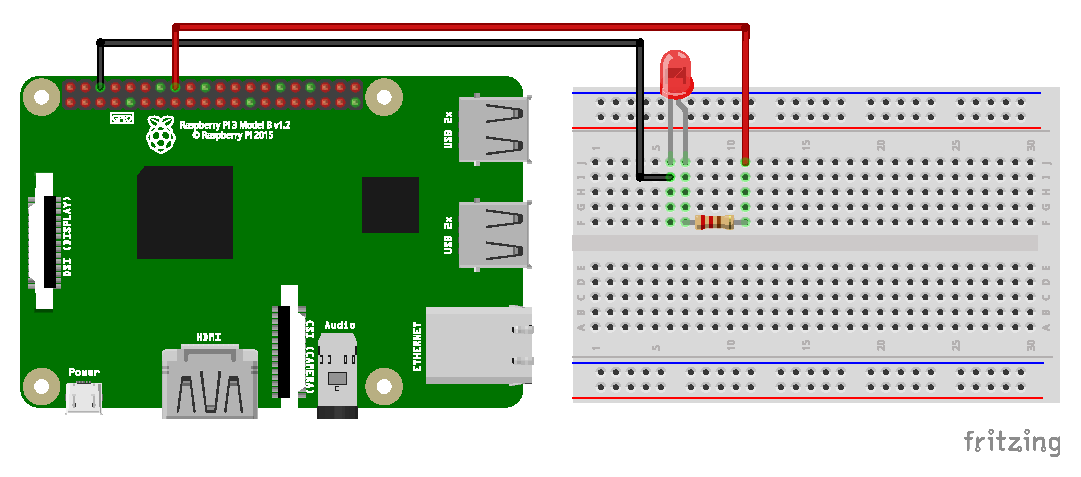
\includegraphics[width=0.95\linewidth]{schemas/led_bb}
        \caption{Схема подключения светодиода}
        \label{fig:led}
    \end{figure}

    Схема подключение сервомотора изображена на рис.~\ref{fig:servo}.
    Для подключения данного устройства необходимо добавить дополнительное питание.

    \begin{figure}[H]
        \centering
        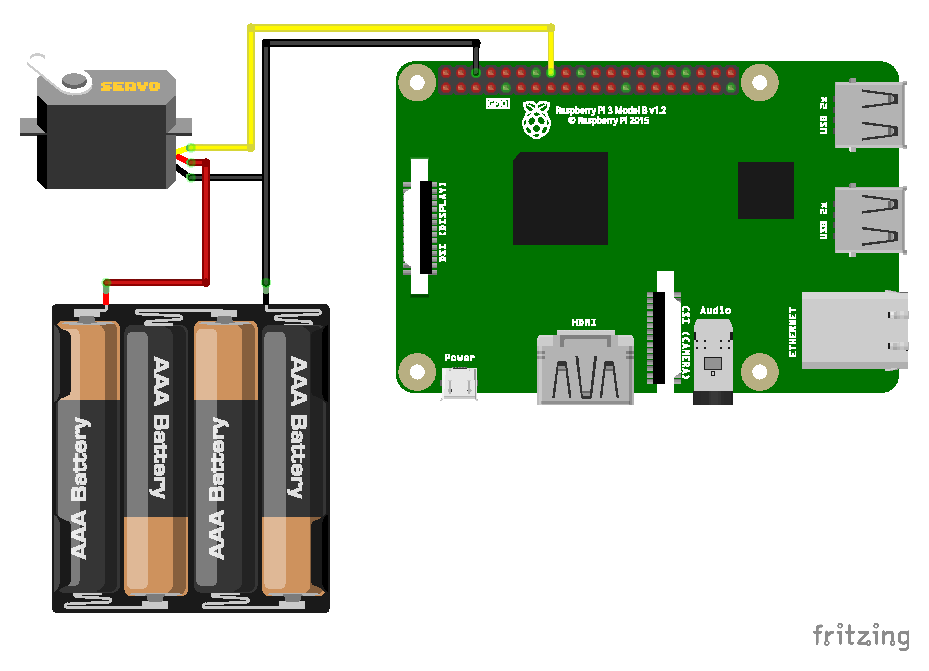
\includegraphics[width=0.95\linewidth]{schemas/servo_bb}
        \caption{Схема подключения сервомотора}
        \label{fig:servo}
    \end{figure}

    Камера подключается посредством USB.

    \subsection{Код управления поиска красных круглых объектов}

    Для работы с устройством был написан промежуточный модуль, который облегчает взаимодействие с железом и выполняет однотипные действия по настройке платы и инициализации пинов.

    {\small \VerbatimInput{../raspberrypi_lab_01/hardware.py}}

    Далее представлен код работы детектора красных кругов.
    Приложение в цикле получает изображение, подготавливает его и ищет целевые объекты.
    При нахождении подсвечивает их зеленым кругом.
    Кроме того, на светодиод отправляется команда в зависимости от наличия цели.
    Если самая крупная цель находится не по центру изображения, отправляется команда на поворот камеры.

    {\small \VerbatimInput{../raspberrypi_lab_01/task_01_red_detection.py}}

    \subsection{Реализация нейронной сети MobileNet}

    Далее представлен код, реализующий поиск объектов с помощью MobileNet.
    При детектировании такого объекта выделяется область данного объекта и добавляется подпись с вероятностью принадлежности к определенному классу.

    {\small \VerbatimInput{../raspberrypi_lab_01/task_02_mobile_net.py}}


    \section{Исходные коды}

    Исходные коды доступны на \href{https://github.com/AsciiShell/hse_hlimds_labs}
    {https://github.com/AsciiShell/hse\_hlimds\_labs}.

    Pull request работы \href{https://github.com/AsciiShell/hse_hlimds_labs/pull/1}
    {https://github.com/AsciiShell/hse\_hlimds\_labs/pull/1}.

    Релизы \href{https://github.com/AsciiShell/hse_hlimds_labs/releases}
    {https://github.com/AsciiShell/hse\_hlimds\_labs/releases}.


    \section{Выводы по работе}

    В ходе работы получен опыт работы с Raspberry Pi.
    Был получен опыт написания кода для управления периферийными устройствами.
    Был получен опыт работы с библиотекой opencv.
    Изучены и созданы программы для обработки видеоряда с помощью данной библиотеки.
    Была написана программа для детектирования красных круглых объектов на видео.
    Был создан модуль для управления периферийными устройствами.
    Была применена модель MobileNet для детектирования объектов на видео.
    Итоговый проект был протестирован на плате.

\end{document} % конец документа
